\begin{figure}[H]\centering
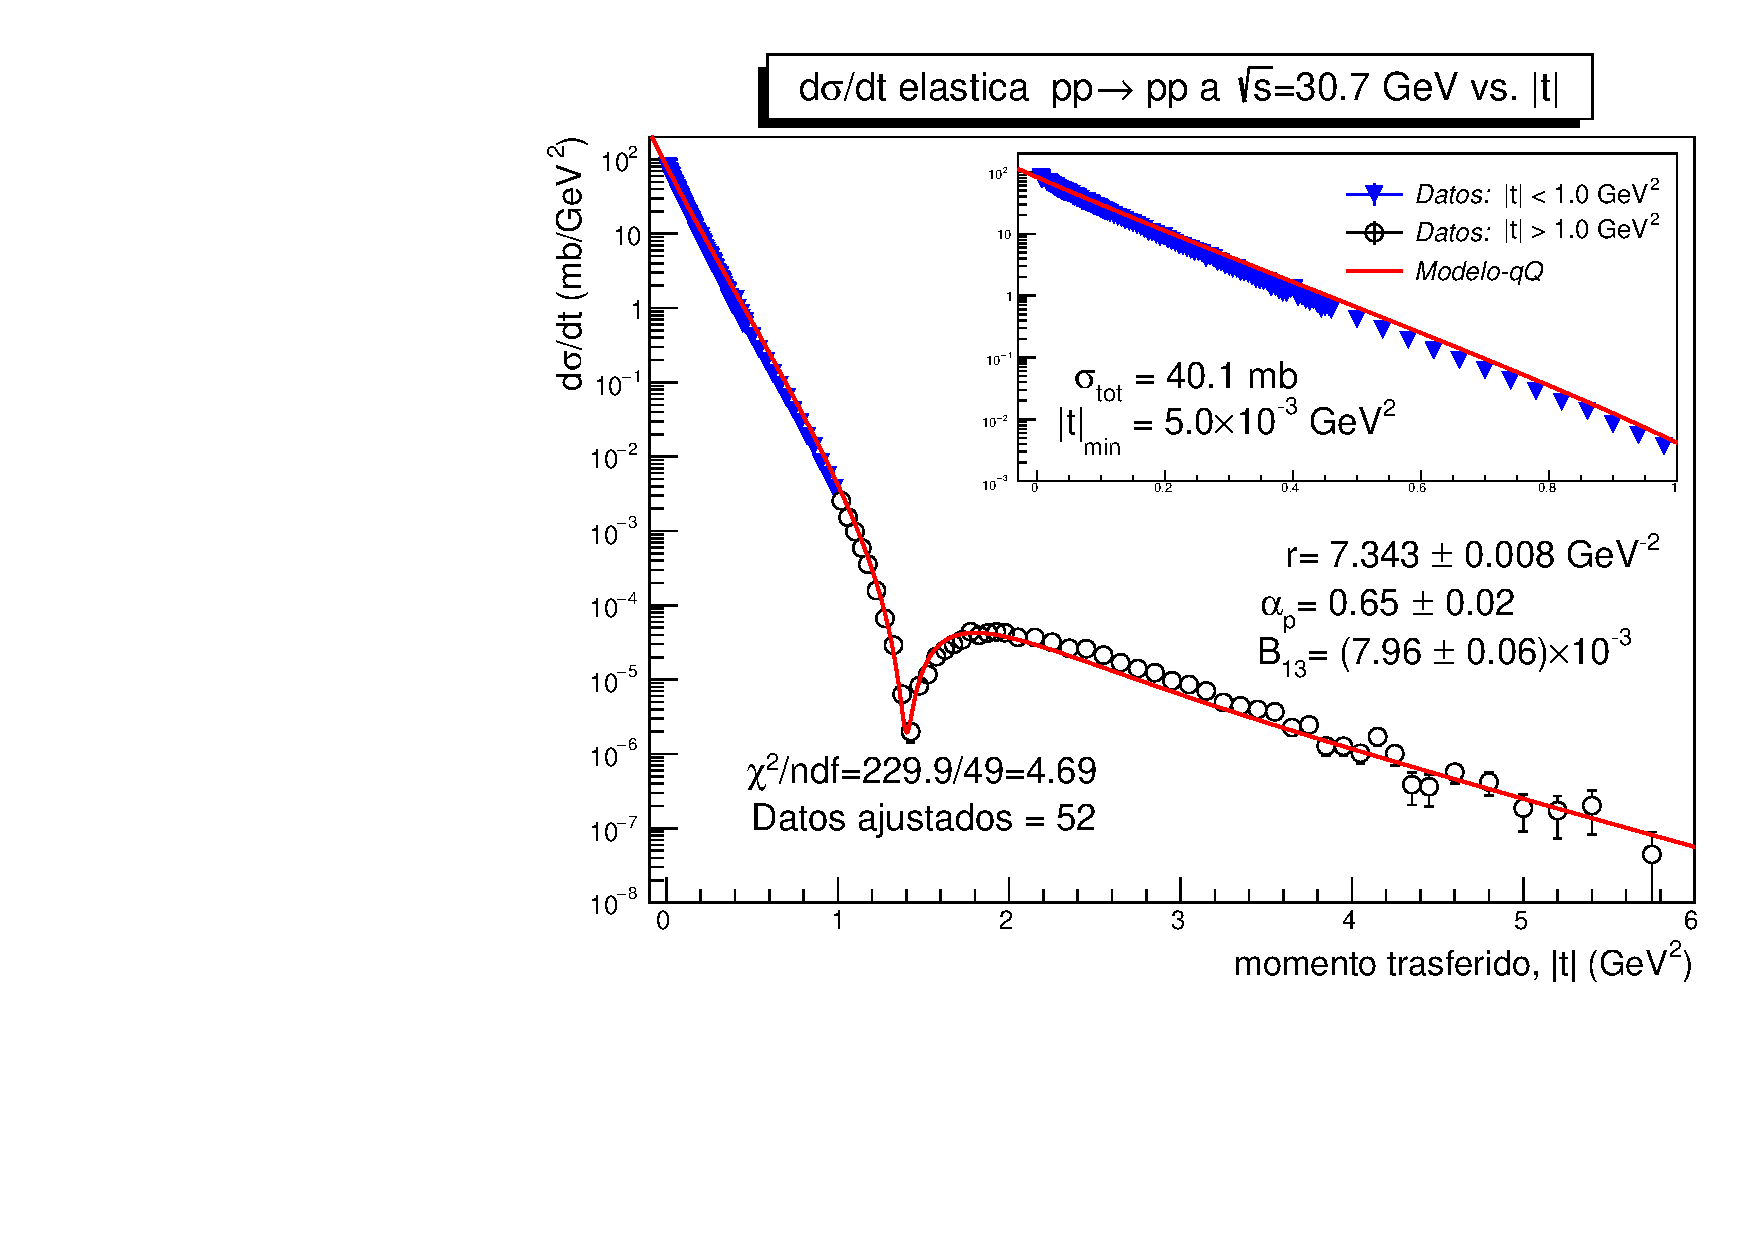
\includegraphics[width=8cm]{/home/alejandro/Escritorio/articulodoc/graficas/ajuste30pp.pdf}
\caption{\mismall Se muestra el ajuste a los datos de sección eficaz diferencial elástica en colisiones prot\'on-prot\'on a $\sqrt{s}=30\textup{.}7$ GeV. La curva es el modelo $qQ_{-}$ con pomer\'on elástico para el intervalo de ajuste 1.0 GeV$^2<|t|<\textup{6.0 GeV}^2$.}
\label{lafig_8}
\end{figure}\vskip -0.05cm
\begin{figure}[H]\centering
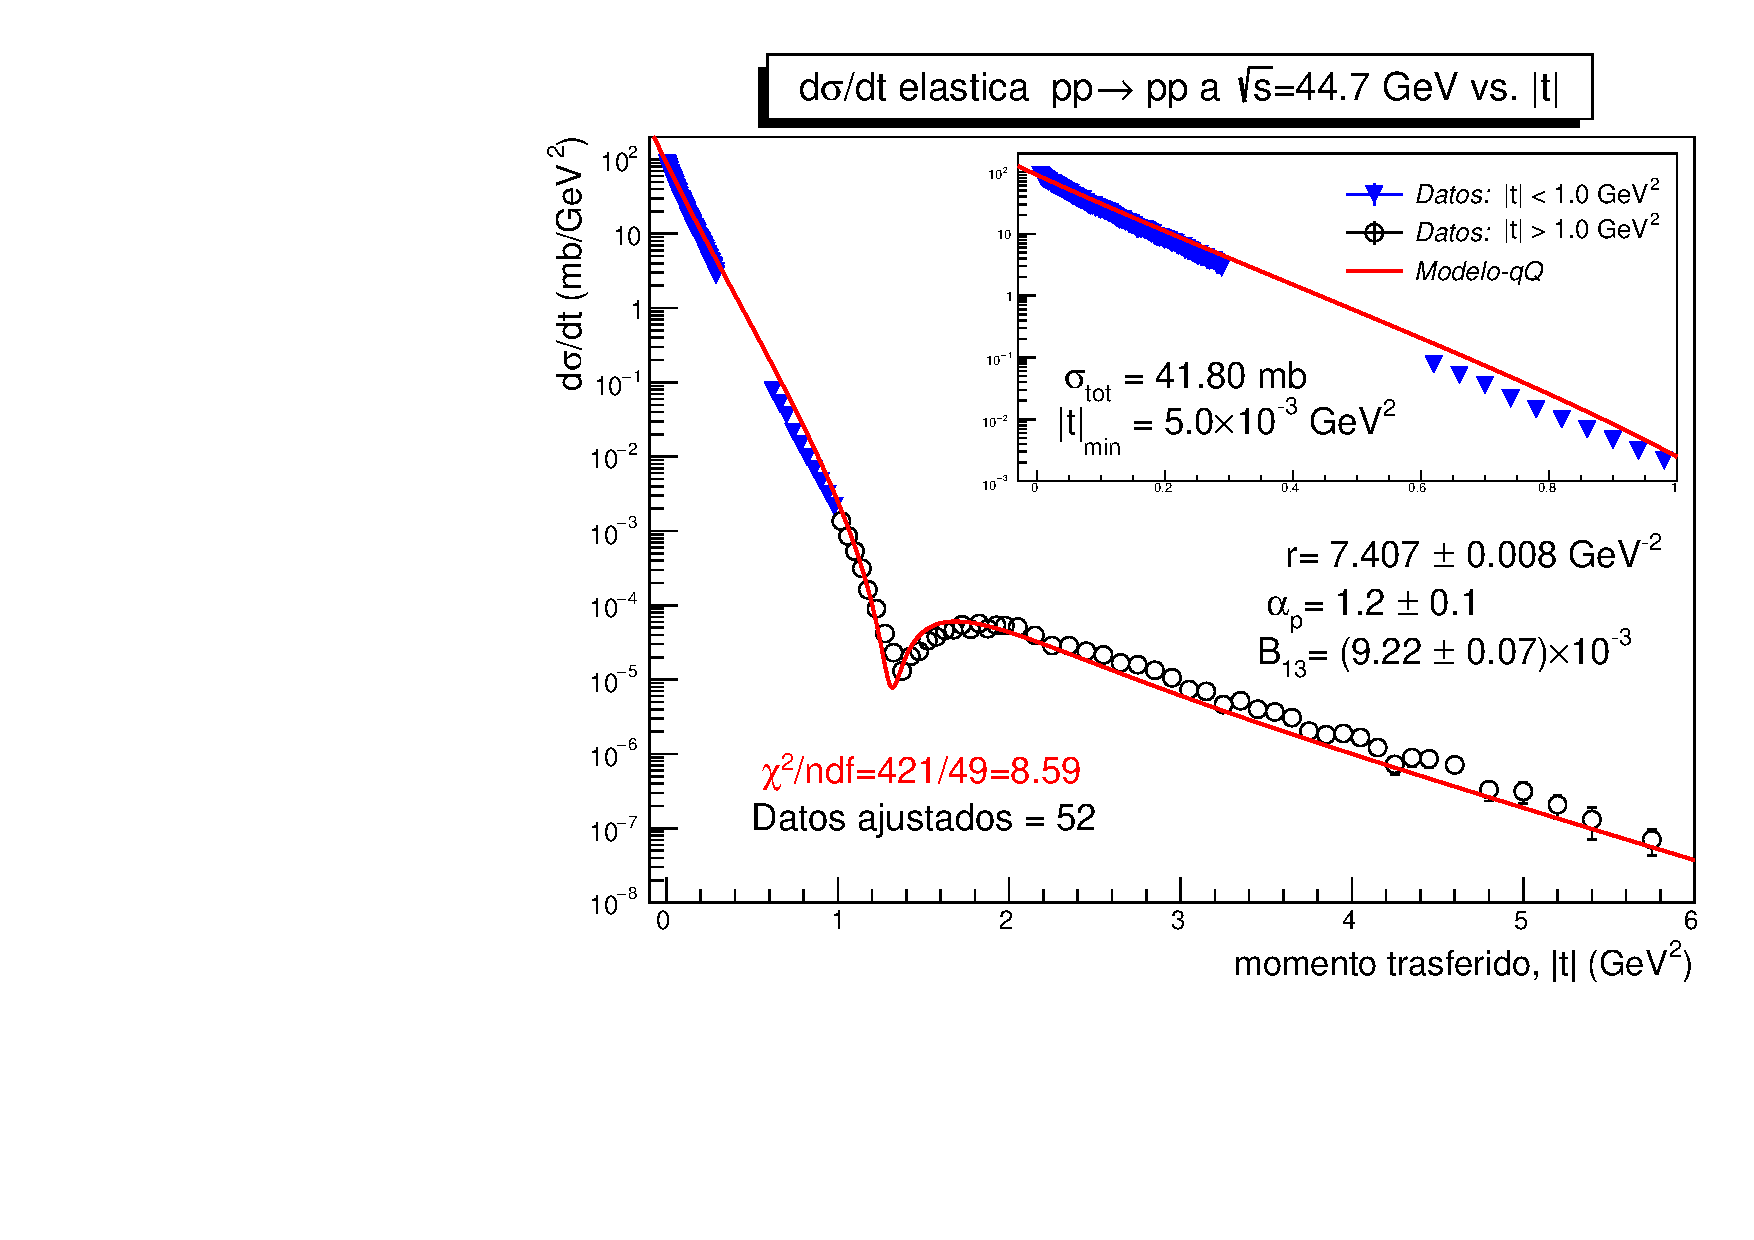
\includegraphics[width=8cm]{/home/alejandro/Escritorio/articulodoc/graficas/ajuste44pp.pdf}
\caption{\mismall Se muestra el ajuste a los datos de sección eficaz diferencial elástica en colisiones prot\'on-prot\'on a $\sqrt{s}=44\textup{.}7$ GeV. La curva es el modelo $qQ_{-}$ con pomer\'on elástico para el intervalo de ajuste 1.0 GeV$^2<|t|<\textup{6.0 GeV}^2$.}
\label{lafig_9}
\end{figure}\vskip -0.05cm
\begin{figure}[H]\centering
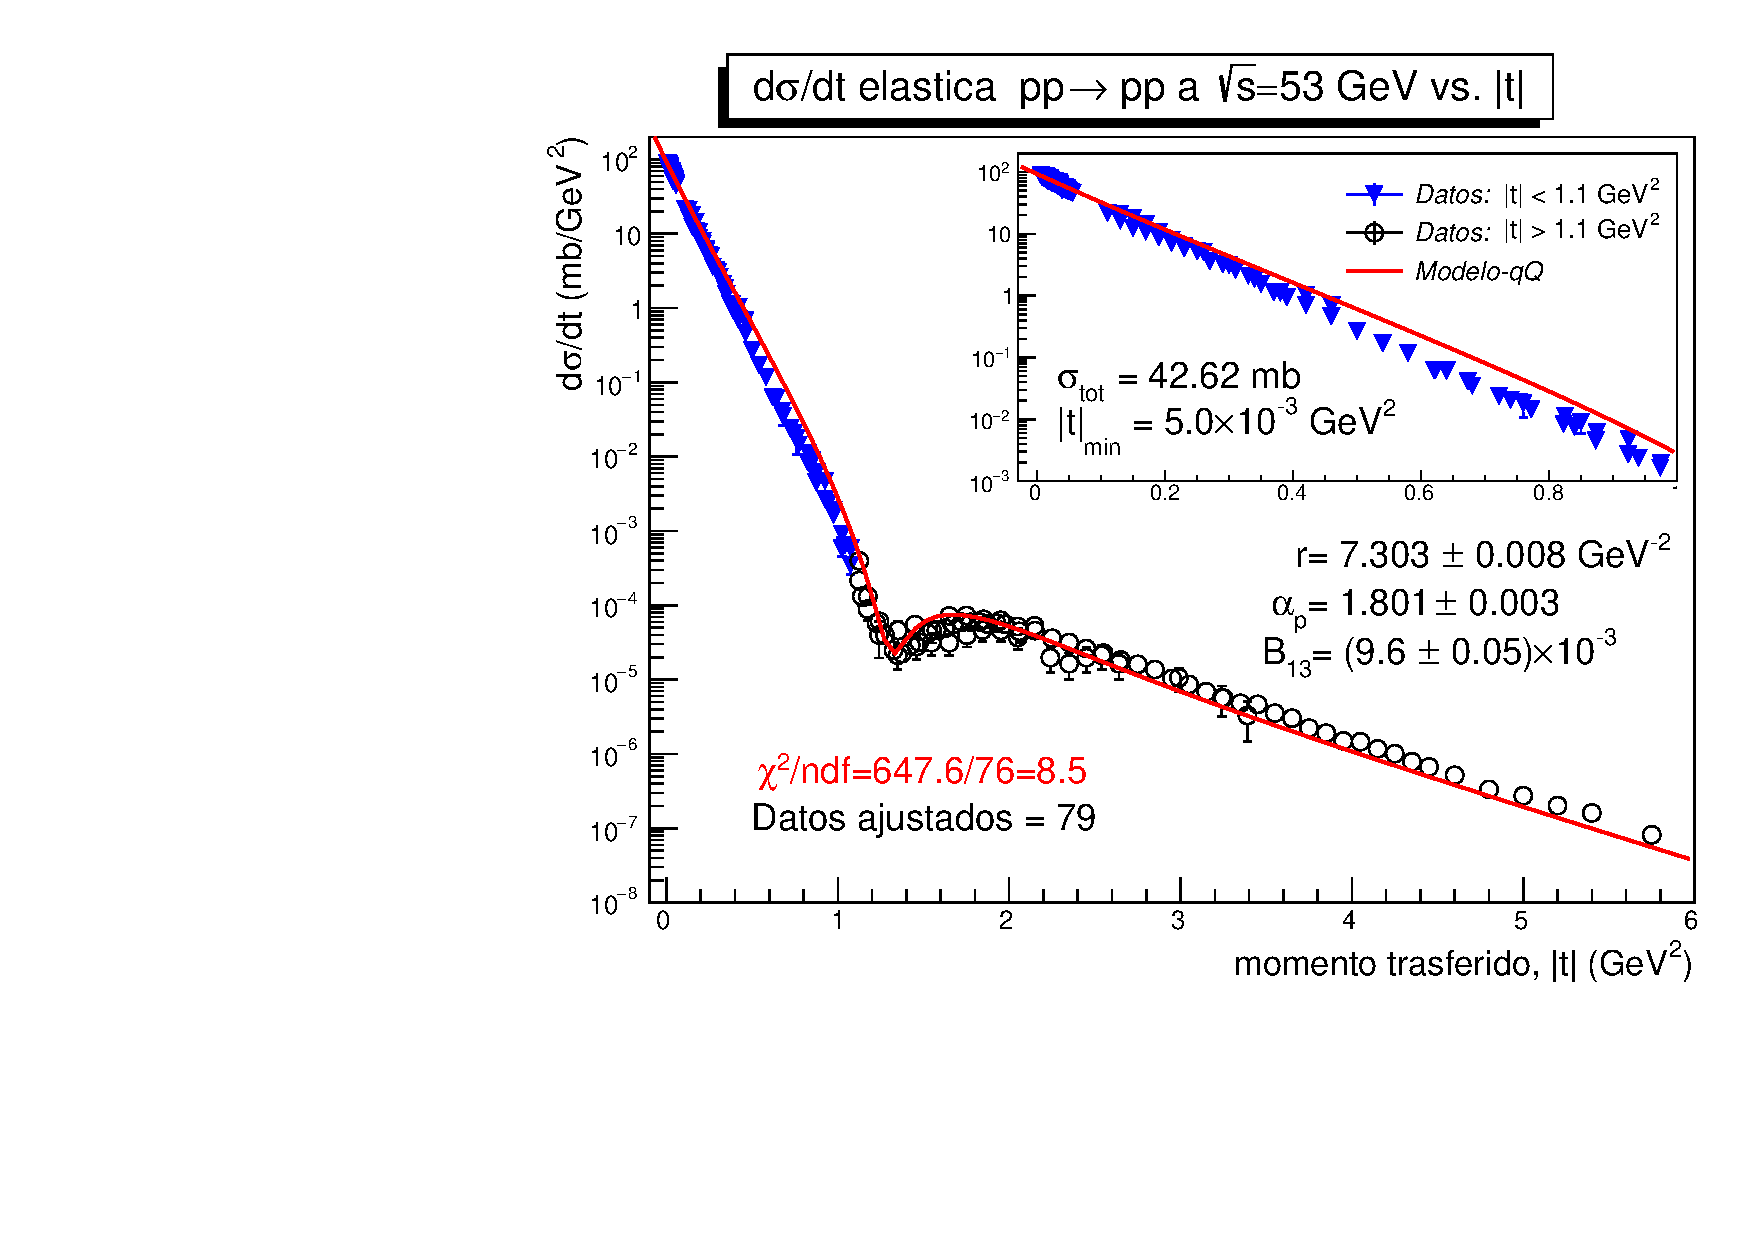
\includegraphics[width=8cm]{/home/alejandro/Escritorio/articulodoc/graficas/ajuste53pp.pdf}
\caption{\mismall Se muestra el ajuste a los datos de sección eficaz diferencial elástica en colisiones prot\'on-prot\'on a $\sqrt{s}=53\textup{.}0$ GeV. La curva es el modelo $qQ_{-}$ con pomer\'on elástico para el intervalo de ajuste 1.0 GeV$^2<|t|<\textup{6.0 GeV}^2$.}
\label{lafig_10}
\end{figure}
\begin{figure}[H]\centering
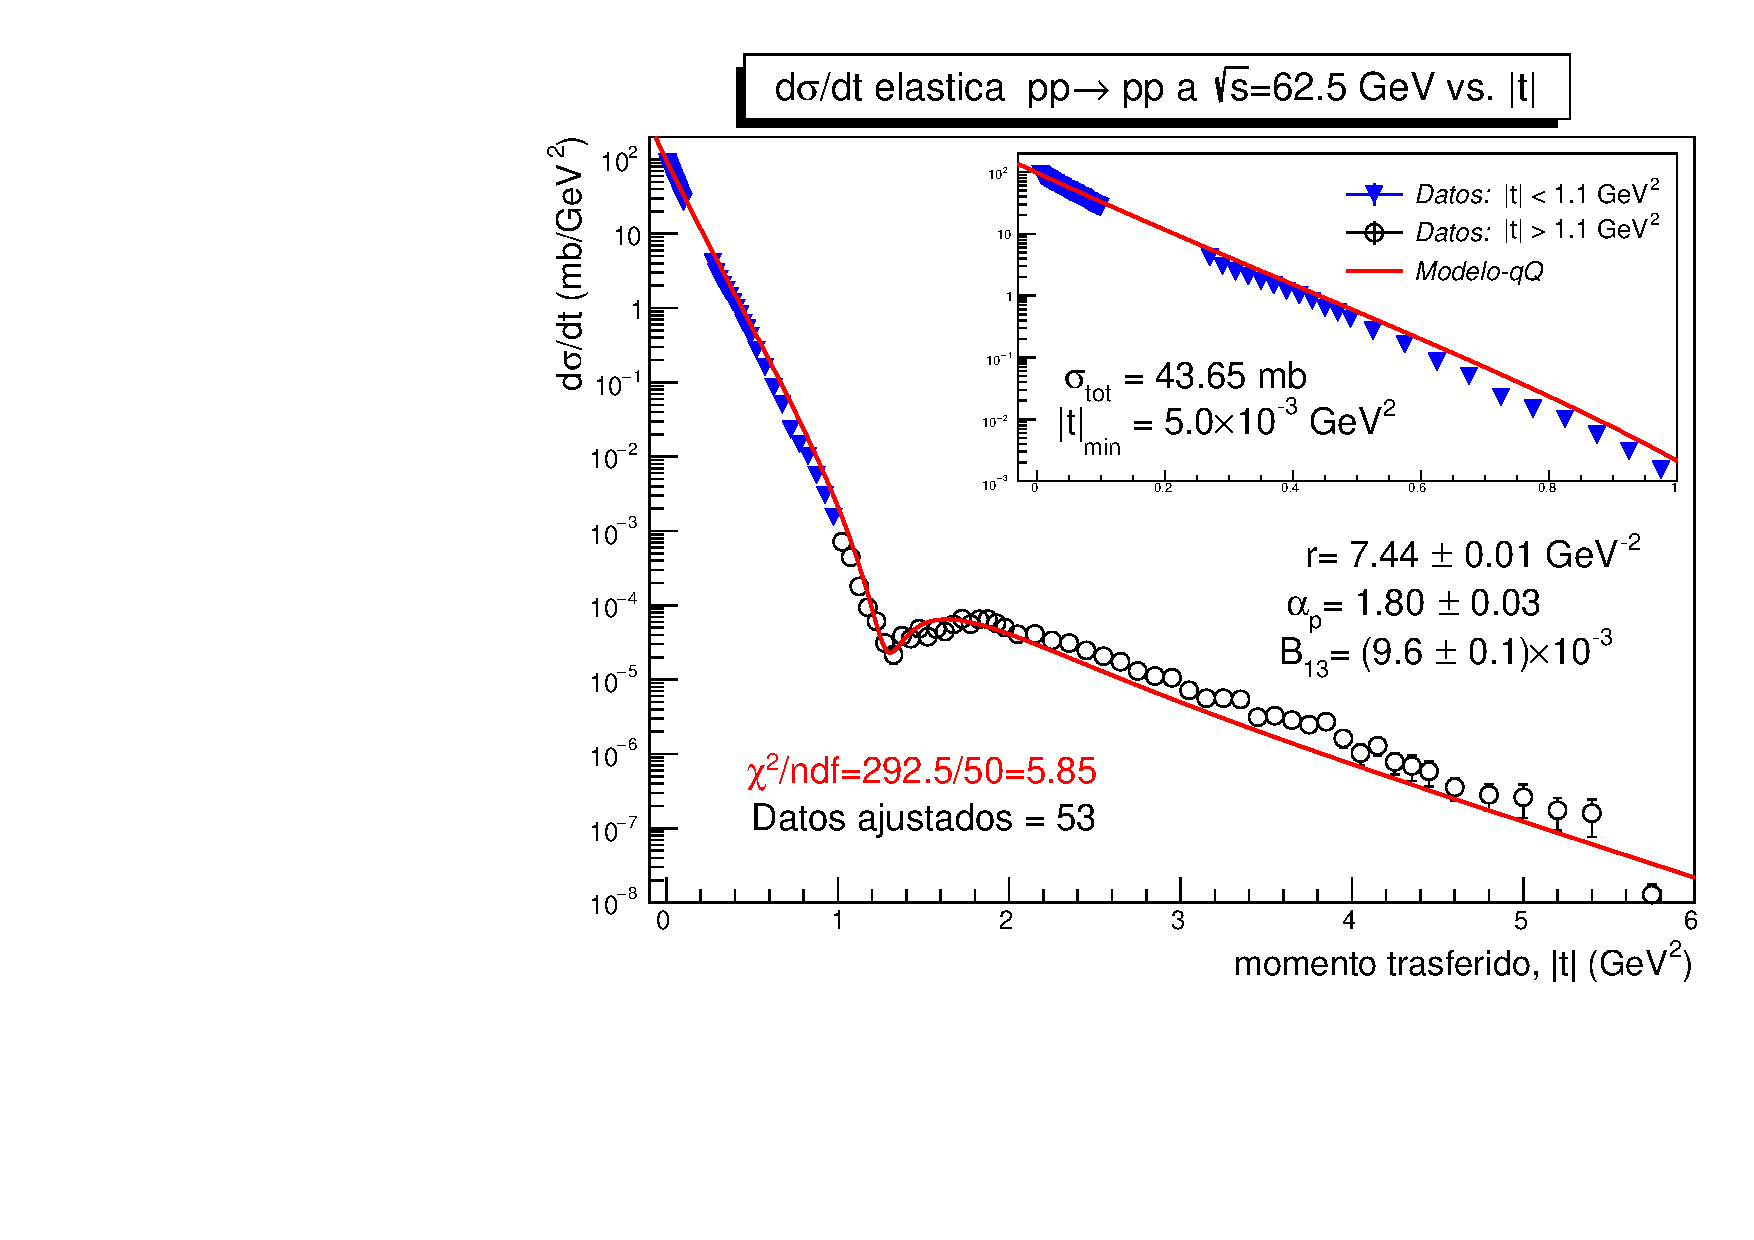
\includegraphics[width=8cm]{/home/alejandro/Escritorio/articulodoc/graficas/ajuste62pp.pdf}
\caption{La dependencia de $\alpha'$ en GeV$^{-2}$ del logaritmo del logaritmo del logaritmo de $\left(\sqrt{s/s_{0}}\right)$.}
\label{lafig_11}
\end{figure}%\vskip -1cm
\begin{figure}[H]\centering
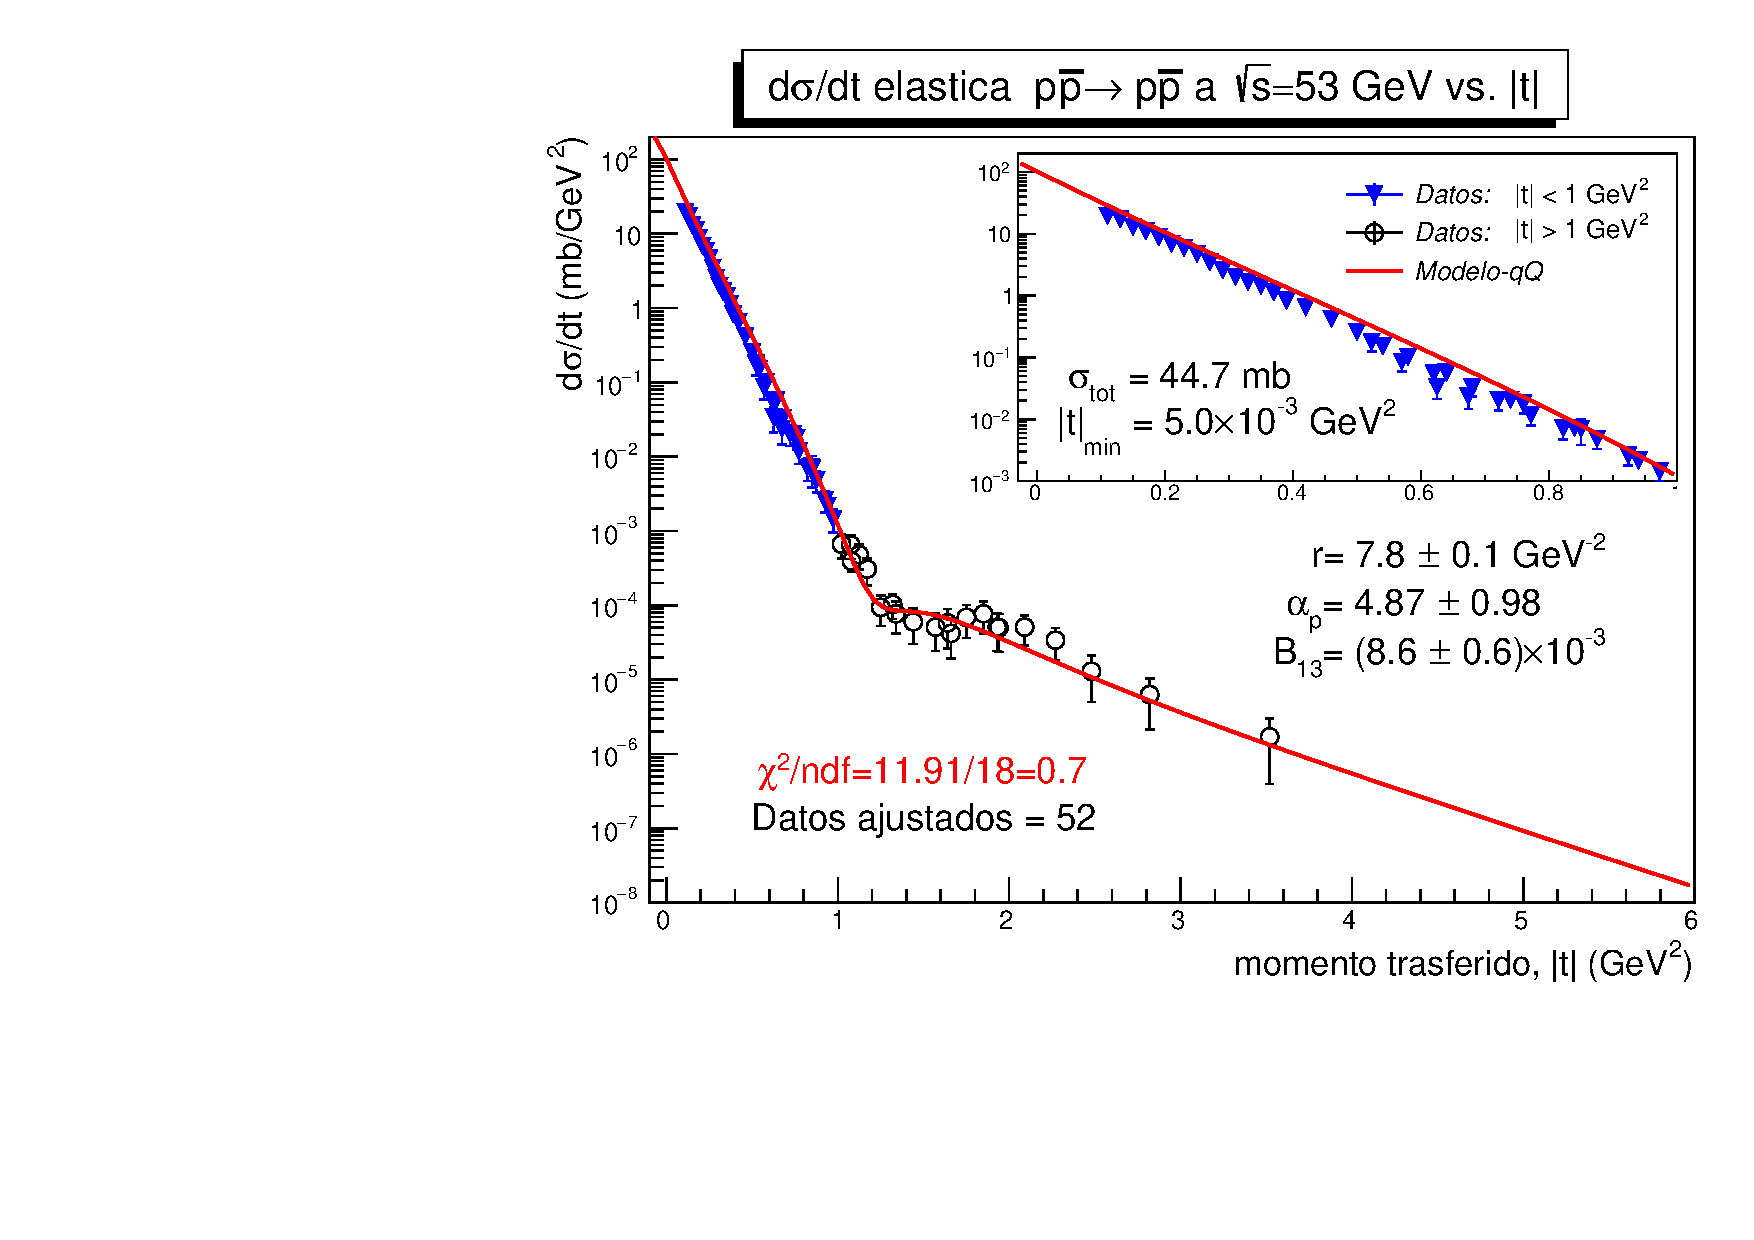
\includegraphics[width=8cm]{/home/alejandro/Escritorio/articulodoc/graficas/ajuste53pbar_p.pdf}
\caption{La dependencia de $\alpha'$ en GeV$^{-2}$ del logaritmo del logaritmo del logaritmo de $\left(\sqrt{s/s_{0}}\right)$.}
\label{lafig_12}
\end{figure}%\vskip -0.cm
\begin{figure}[H]\centering
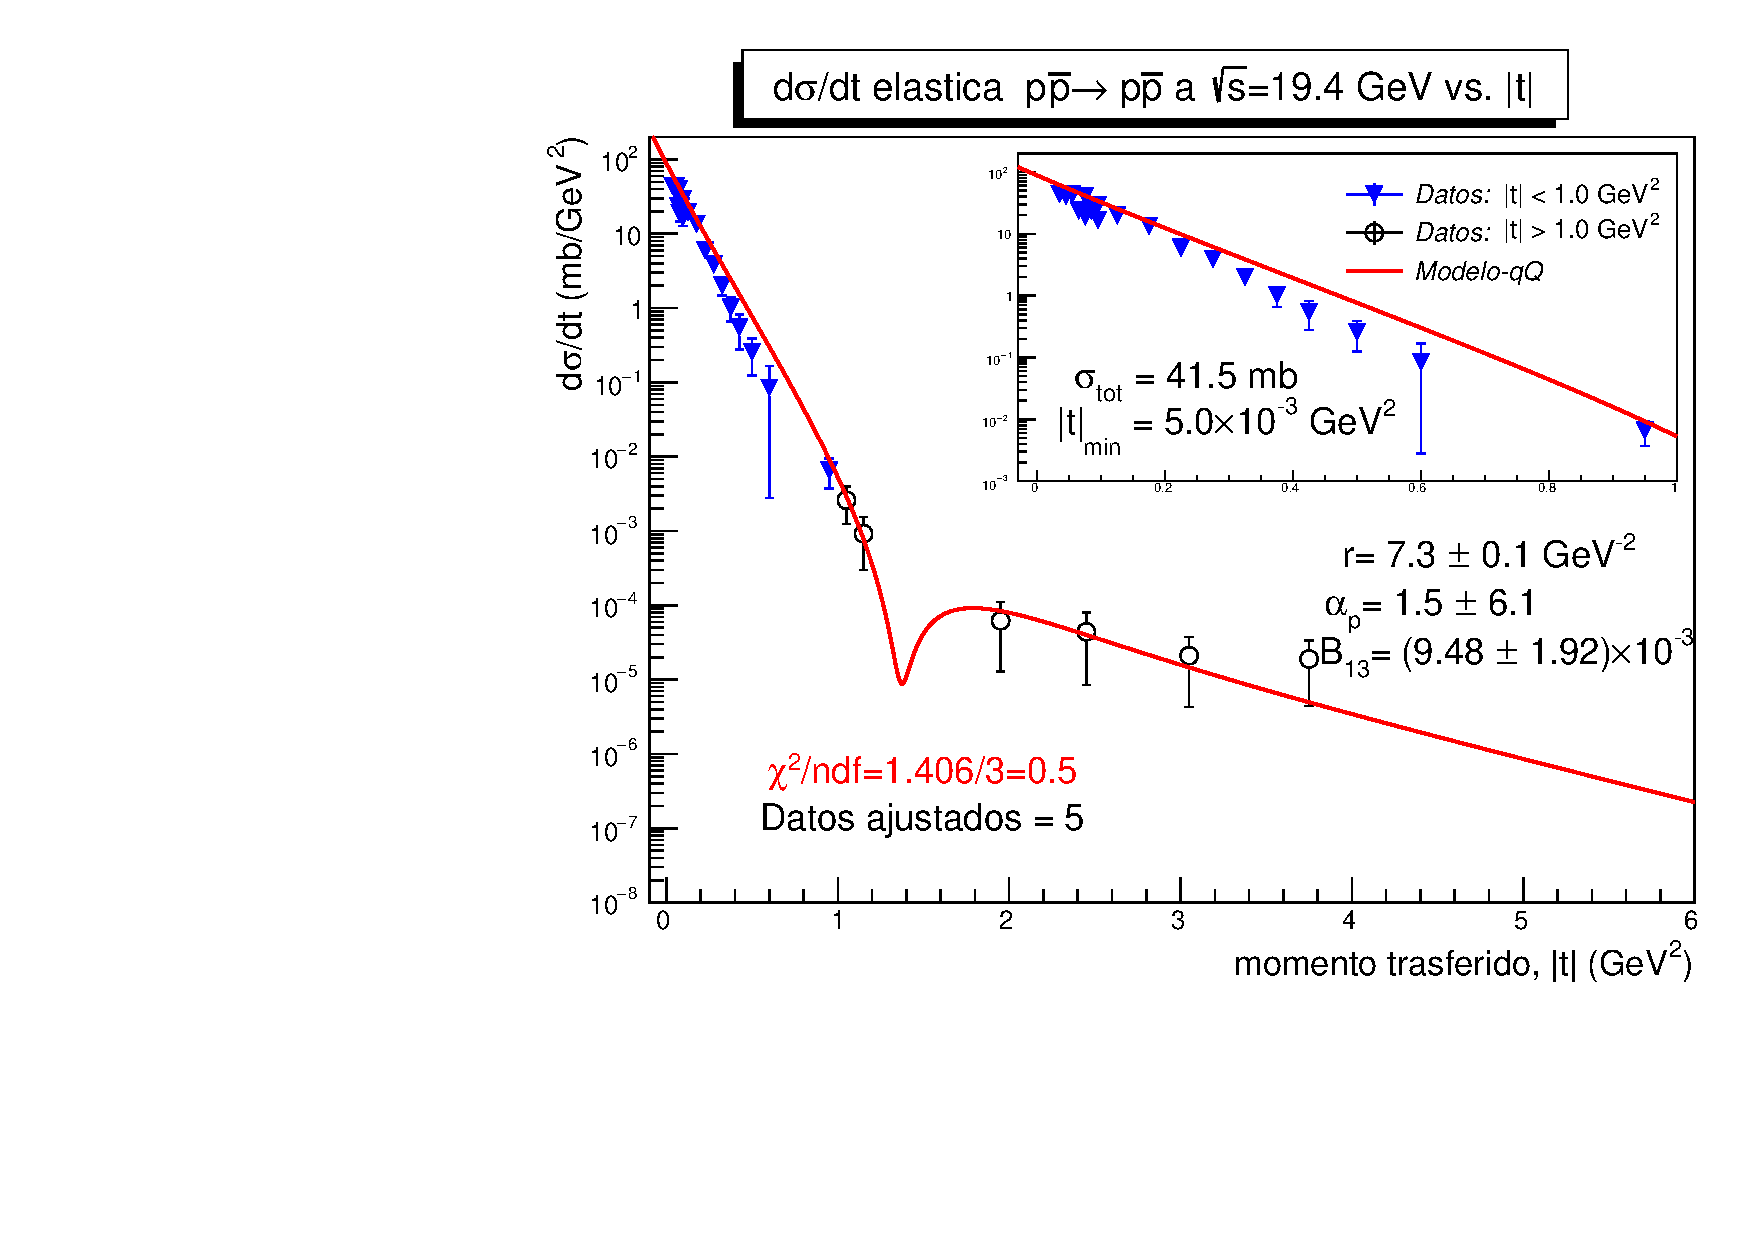
\includegraphics[width=8cm]{/home/alejandro/Escritorio/articulodoc/graficas/ajuste19pbar_p.pdf}
\caption{La dependencia de $\alpha'$ en GeV$^{-2}$ del logaritmo del logaritmo del logaritmo de $\left(\sqrt{s/s_{0}}\right)$.}
\label{lafig_13}
\end{figure}%